% This must be in the first 5 lines to tell arXiv to use pdfLaTeX, which is strongly recommended.
\pdfoutput=1
% In particular, the hyperref package requires pdfLaTeX in order to break URLs across lines.
\newcommand{\DatasetName}{\textsc{NSF-SciFy}}
\newcommand{\DatasetNameMatSci}{\textsc{NSF-SciFy-MatSci}}
\newcommand{\NSF}{National Science Foundation}
\documentclass[11pt]{article}

\usepackage[table]{xcolor}
% Change "review" to "final" to generate the final (sometimes called camera-ready) version.
% Change to "preprint" to generate a non-anonymous version with page numbers.
\usepackage[preprint]{acl}

% Standard package includes
\usepackage{times}
\usepackage{latexsym}
\usepackage{hyperref}
% For proper rendering and hyphenation of words containing Latin characters (including in bib files)
\usepackage[T1]{fontenc}
% For Vietnamese characters
% \usepackage[T5]{fontenc}
% See https://www.latex-project.org/help/documentation/encguide.pdf for other character sets

% This assumes your files are encoded as UTF8
\usepackage[utf8]{inputenc}

% This is not strictly necessary, and may be commented out,
% but it will improve the layout of the manuscript,
% and will typically save some space.
\usepackage{microtype}

% This is also not strictly necessary, and may be commented out.
% However, it will improve the aesthetics of text in
% the typewriter font.
\usepackage{inconsolata}

%Including images in your LaTeX document requires adding
%additional package(s)
\usepackage{graphicx}

% If the title and author information does not fit in the area allocated, uncomment the following
%
%\setlength\titlebox{<dim>}
%
% and set <dim> to something 5cm or larger.

\definecolor{darkgreen}{rgb}{0,0.5,0}
\usepackage{enumitem}
\usepackage{todonotes}
\usepackage{booktabs}

\usepackage[symbol]{footmisc}
\usepackage{mdframed}
\usepackage{listings}
\lstset{
basicstyle=\small\ttfamily,
columns=flexible,
breaklines=true
}

\usepackage{amsmath}

\title{\DatasetName: Mining the NSF Awards Database for Scientific Claims}

% Author information can be set in various styles:
% For several authors from the same institution:
% \author{Author 1 \and ... \and Author n \\
%         Address line \\ ... \\ Address line}
% if the names do not fit well on one line use
%         Author 1 \\ {\bf Author 2} \\ ... \\ {\bf Author n} \\
% For authors from different institutions:
% \author{Author 1 \\ Address line \\  ... \\ Address line
%         \And  ... \And
%         Author n \\ Address line \\ ... \\ Address line}
% To start a separate ``row'' of authors use \AND, as in
% \author{Author 1 \\ Address line \\  ... \\ Address line
%         \AND
%         Author 2 \\ Address line \\ ... \\ Address line \And
%         Author 3 \\ Address line \\ ... \\ Address line}

\author{Delip Rao\thanks{Corresponding author, $^\dagger$co-first author}$^\dagger$, Weiqiu You$^\dagger$, Eric Wong, Chris Callison-Burch \\
	    University of Pennsylvania \\
        Philadelphia, PA, USA \\
	    {\tt \{delip, weiqiuy, exwong, ccb\}@seas.upenn.edu} }

%\author{
%  \textbf{First Author\textsuperscript{1}},
%  \textbf{Second Author\textsuperscript{1,2}},
%  \textbf{Third T. Author\textsuperscript{1}},
%  \textbf{Fourth Author\textsuperscript{1}},
%\\
%  \textbf{Fifth Author\textsuperscript{1,2}},
%  \textbf{Sixth Author\textsuperscript{1}},
%  \textbf{Seventh Author\textsuperscript{1}},
%  \textbf{Eighth Author \textsuperscript{1,2,3,4}},
%\\
%  \textbf{Ninth Author\textsuperscript{1}},
%  \textbf{Tenth Author\textsuperscript{1}},
%  \textbf{Eleventh E. Author\textsuperscript{1,2,3,4,5}},
%  \textbf{Twelfth Author\textsuperscript{1}},
%\\
%  \textbf{Thirteenth Author\textsuperscript{3}},
%  \textbf{Fourteenth F. Author\textsuperscript{2,4}},
%  \textbf{Fifteenth Author\textsuperscript{1}},
%  \textbf{Sixteenth Author\textsuperscript{1}},
%\\
%  \textbf{Seventeenth S. Author\textsuperscript{4,5}},
%  \textbf{Eighteenth Author\textsuperscript{3,4}},
%  \textbf{Nineteenth N. Author\textsuperscript{2,5}},
%  \textbf{Twentieth Author\textsuperscript{1}}
%\\
%\\
%  \textsuperscript{1}Affiliation 1,
%  \textsuperscript{2}Affiliation 2,
%  \textsuperscript{3}Affiliation 3,
%  \textsuperscript{4}Affiliation 4,
%  \textsuperscript{5}Affiliation 5
%\\
%  \small{
%    \textbf{Correspondence:} \href{mailto:email@domain}{email@domain}
%  }
%}

\begin{document}
\maketitle
\begin{abstract}

We present \DatasetName, a large-scale dataset for scientific claim extraction derived from the \NSF~(NSF) awards database, comprising over 400K grant abstracts spanning five decades. While previous datasets relied on published literature, we leverage grant abstracts which offer a unique advantage: they capture claims at an earlier stage in the research lifecycle before publication takes effect. We also introduce a new task  to distinguish between existing scientific claims and aspirational research intentions in proposals.Using zero-shot prompting with frontier large language models, we jointly extract 114K scientific claims and 145K investigation proposals from 16K grant abstracts in the materials science domain to create a focused subset called \DatasetNameMatSci. We use this dataset to evaluate 3 three key tasks: (1) technical to non-technical abstract generation, where models achieve high BERTScore (0.85+ F1); (2) scientific claim extraction, where fine-tuned models outperform base models by 100\% relative improvement; and (3) investigation proposal extraction, showing 90\%+ improvement with fine-tuning. We introduce novel LLM-based evaluation metrics for robust assessment of claim/proposal extraction quality. As the largest scientific claim dataset to date -- with an estimated 2.8 million claims across all STEM disciplines funded by the NSF -- \DatasetName~enables new opportunities for claim verification and meta-scientific research. We publicly release all datasets, trained models, and evaluation code to facilitate further research.
\end{abstract}


\section{Introduction}
\begin{figure}[h]
    \centering
    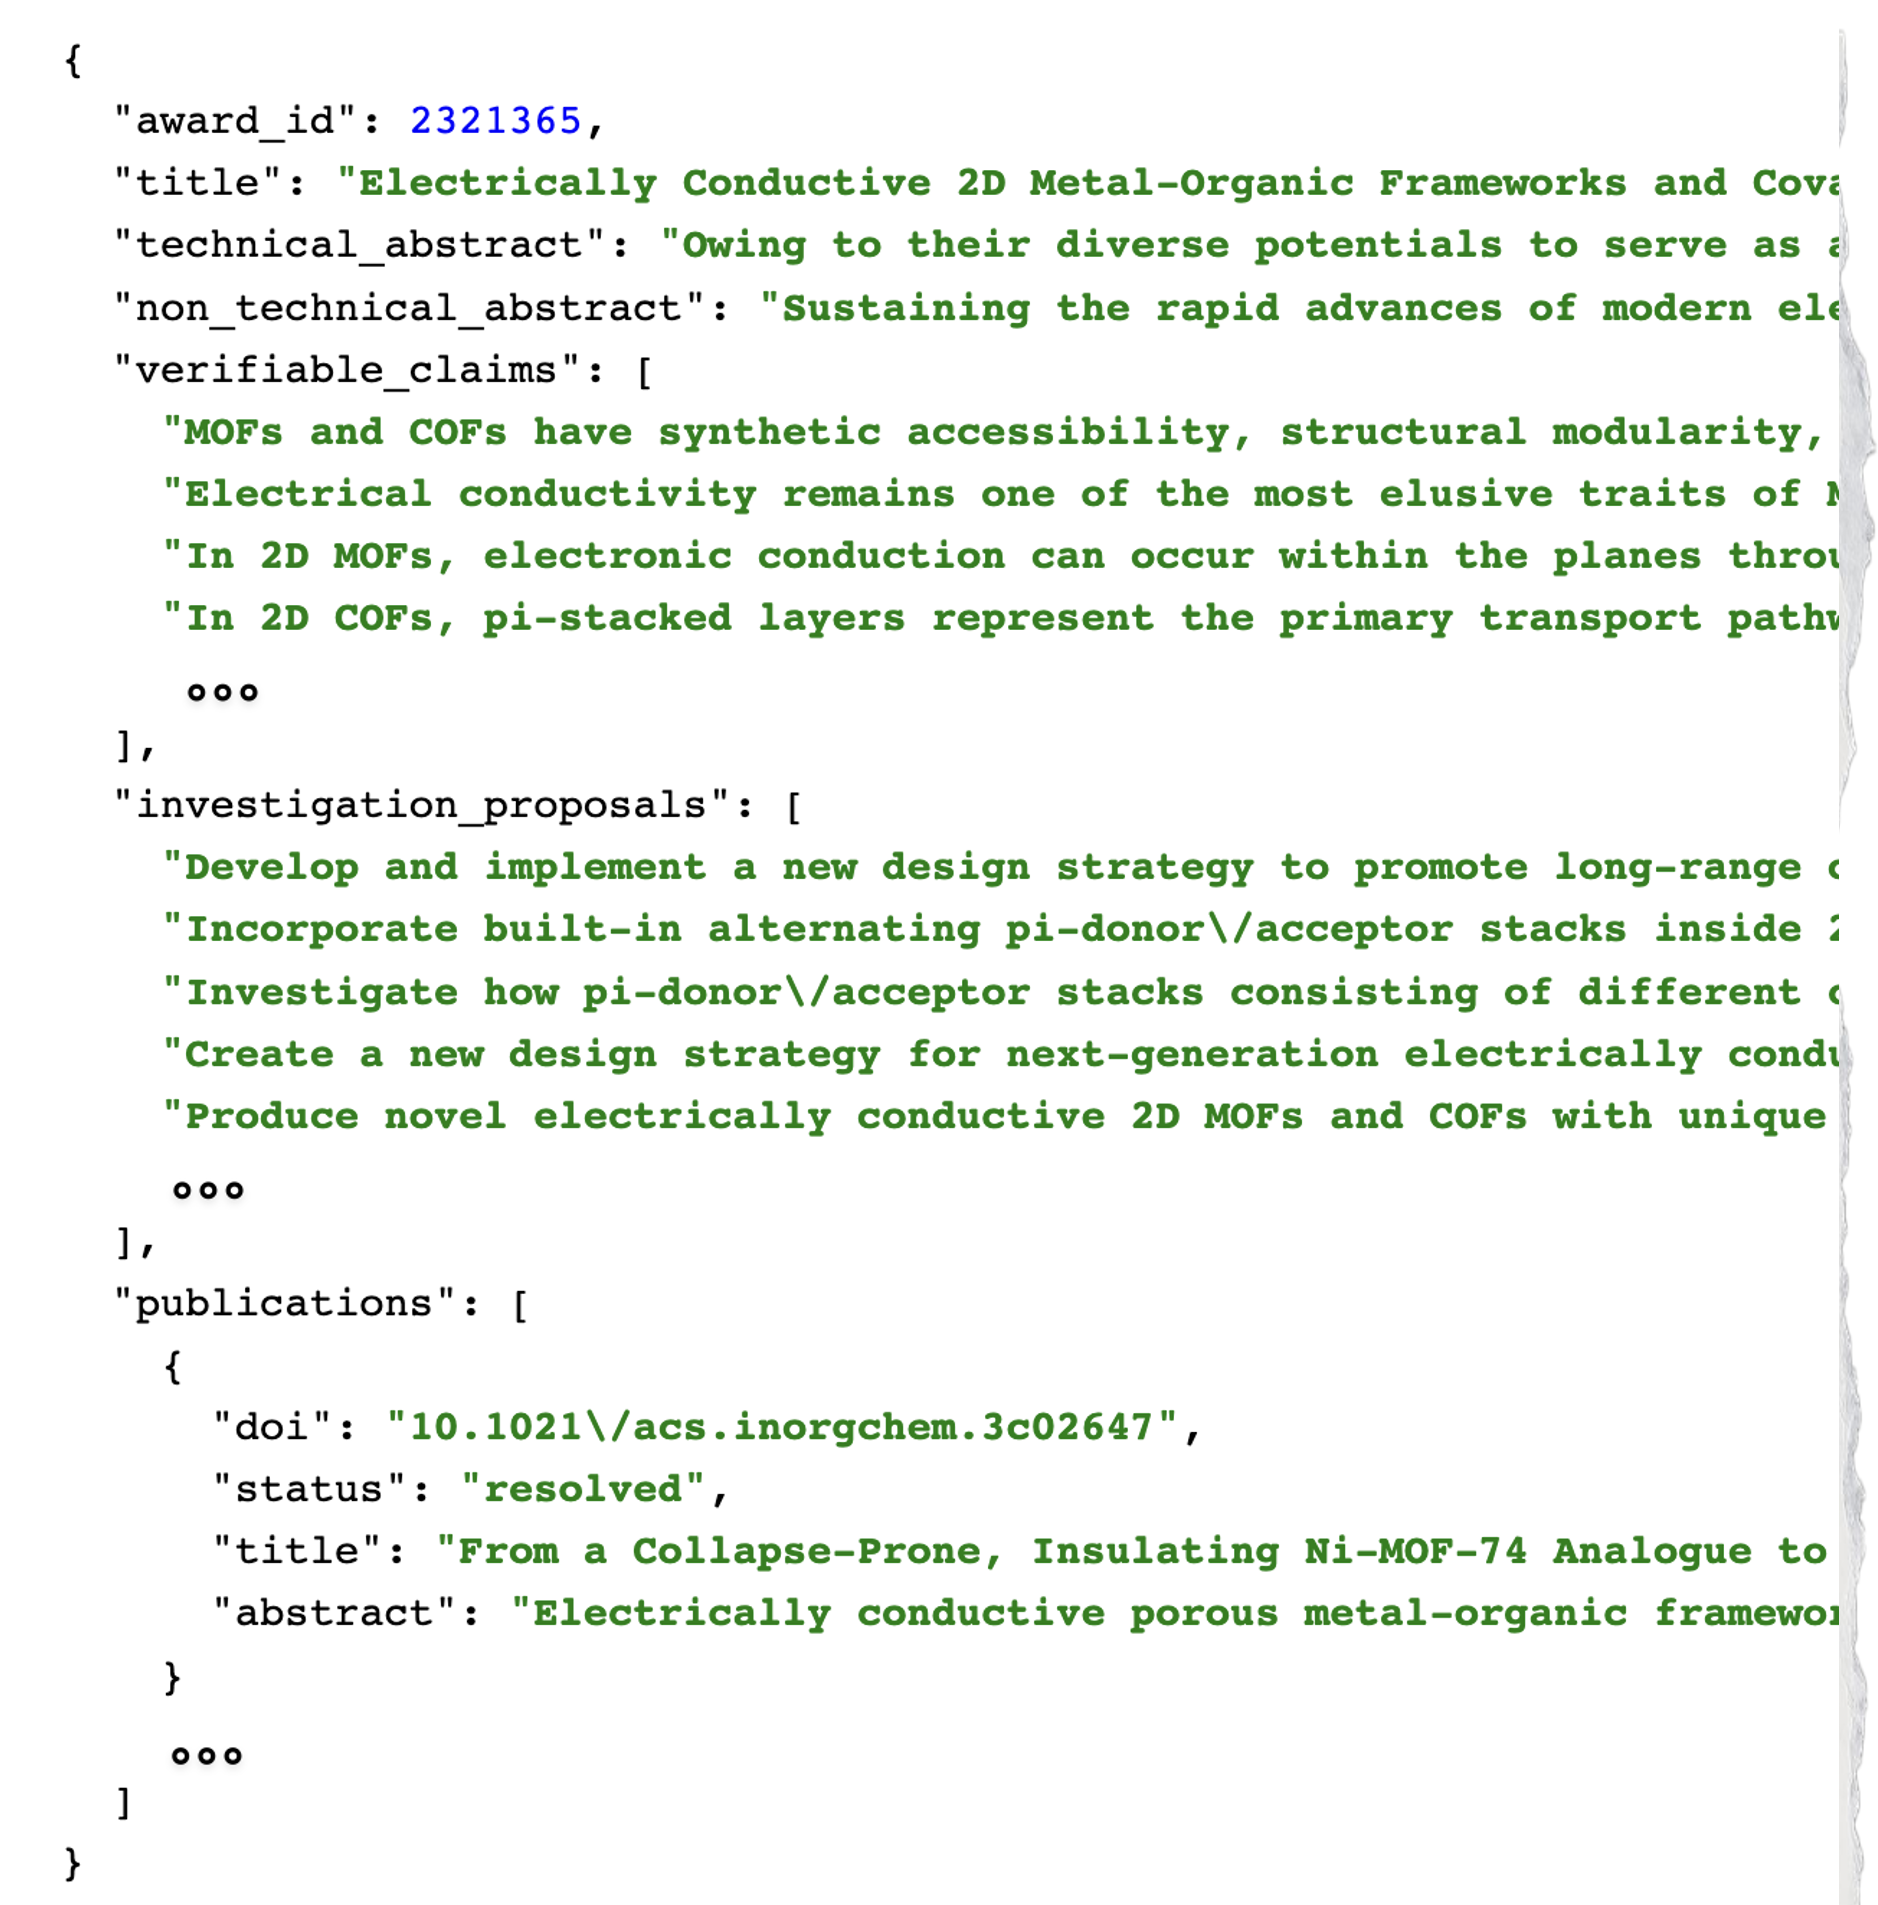
\includegraphics[width=1\linewidth]{images/nsf-scify-sample-record.png}
    \caption{A sample record from our \DatasetName~dataset. Each record contains 1) Award ID and title, 2) NSF Directorate, 3) Technical and non-technical abstracts, 4) Scientific Claims, 5) Investigation Proposals, and 6) Associated publications, when present.}
    \label{fig:sample-record}
\end{figure}
The overall growth rate of scientific publications is estimated to be 4\% annually, with a doubling time of 17 years~\cite{Bornmann2021}. Within this deluge, researchers, reviewers, and the general public struggle to separate substantiated claims from spurious ones—whether it is the ``quantum supremacy'' assertions in computing, the short-lived excitement over LK-99 superconductors\footnote[3]{for an entertaining digression c.f., \url{https://en.wikipedia.org/wiki/LK-99}}, or the misunderstanding surrounding microplastic leaches from black plastic spatulas\footnote[4]{c.f., \url{https://nationalpost.com/news/canada/black-plastic}}. Manual verification of ever growing body of scientific claims has become intractable, yet the economic and societal consequences of unverified  claims are increasingly severe. 

\begin{table*}[t]
\centering
\small
\begin{tabular}{@{}lrrll@{}}
\toprule
\textbf{Dataset} & \textbf{\# claims} & \textbf{\# docs} & \textbf{Evidence Source} & \textbf{Domain} \\
\midrule
SciFACT~\cite{wadden-etal-2020} & 1.4K & 5K & Research papers & Biomedical \\
\hline
PubHEALTH~\cite{kotonya-toni-2020}& 11.8K & 11.8K & Fact-checking sites & Public health \\
\hline
CLIMATE-FEVER~\cite{diggelmann-etal-2020} & 1.5K & 7.5K & Wikipedia articles & Climate change \\
\hline
HealthVer~\cite{sarrouti-etal-2021}& 1.8K & 738 & Research papers & Healthcare \\
\hline
COVID-Fact~\cite{saakyan-etal-2021}& 4K & 4K & Research, news & COVID \\
\hline
CoVERT~\cite{mohr-etal-2022}& 300 & 300 & Research, news & Biomedical \\
\hline
SciFACT-Open~\cite{wadden-etal-2022}& 279 & 500K & Research papers & Biomedical \\
\midrule
\textbf{\DatasetNameMatSci~(ours)} & \textbf{114K} & \textbf{16K} & \textbf{NSF award abstracts} & \textbf{Material Science} \\
\hline
\textbf{\DatasetName~(ours)} & \textbf{2.8M}\footnotemark[1] & \textbf{400K} & \textbf{NSF award abstracts} & \textbf{All Science \& Math} \\
\bottomrule
\end{tabular}
\caption{This table comparison clearly illustrates the scale advantage of NSF-SciFy over existing scientific claim verification datasets. While previous datasets like SciFACT and PubHEALTH contain at most thousands of claims from published research papers or fact-checking sources, our \DatasetNameMatSci~dataset contributes 114K claims from 16K materials science grant abstracts. The full \DatasetName~dataset represents an order-of-magnitude increase with an estimated 2.8M claims across 400K abstracts spanning all science \& math disciplines. This work introduces grant abstracts as a novel, untapped source for scientific claim extraction, complementing existing approaches that focus on published literature, news articles, or social media content.}
\label{tab:datasets}
\end{table*}

\citet{wadden-etal-2020} introduced the task of scientific claim verification with the SciFACT dataset, focusing primarily on automatic verification of scientific claims. Follow up works (see Section~\ref{sec:related-work} for a detailed account) have mostly focused on the healthcare, building datasets from scientific publications, and modest-sized dataset creation. In this work, we relax all of these aspects and look at building at least an order of magnitude large-scale scientific claim dataset covering all of basic science. We envision building of such large-scale, scientific claim datasets to help future work on robust scientific claim verification systems. \footnotetext[1]{This is an estimate. Future versions of this preprint will be updated with an exact number once we finish large-scale processing.}

We introduce \DatasetName, a comprehensive dataset of claims and investigation proposals extracted from National Science Foundation (NSF) award abstracts. We choose NSF abstracts as our source material for several reasons:

\begin{enumerate}[noitemsep,topsep=0pt]
\item NSF is a primary driver of U.S. scientific innovation, funding approximately 25\% of all federally supported basic research, spanning the entirety of science and math areas, with an annual budget of \$9.9 billion (FY 2023). Any claim dataset derived from the NSF awards database should faithfully represent the scientific Zeitgeist. 
\item NSF's rigorous subject matter expert-review process provides an high-quality filter for the claims made in funded proposals.
\item The public availability and permissive usage terms of the NSF awards database makes it an excellent resource for open science research.
\item Previous datasets on scientific claims have been derived from scientific papers, but claims in scientific grants, and particularly investigation proposals, remain unstudied.
\end{enumerate}

While not this focus of this paper, grant award abstracts, additionally, provide a unique opportunity to study the relationship between what researchers claim and what they propose to investigate. This could offer valuable insights into scientific practice and the evolution of research questions.

In this paper, we make the following contributions: (1) We introduce \DatasetName, the largest scientific claim dataset to date with an estimated 2.8M claims extracted from 400K NSF award abstracts, establishing grant proposals as a novel source for scientific claim extraction; (2) As a precursor to \DatasetName~and, a current offering, we create \DatasetNameMatSci~focusing exclusively on materials science with 114K extracted claims from 16K abstracts. This is the first materials science claim dataset and, in number of extracted claims, this alone is an order of magnitude bigger than the largest publicly available claim dataset; (3) We develop a zero-shot prompting approach for joint extraction of scientific claims and investigation proposals as a scalable way to bootstrap large-scale scientific claim datasets; (4) We present novel evaluation metrics for claim/proposal extraction based on LLM judgments, showing that fine-tuned models significantly outperform base models; and (5) Finally, we release all datasets and trained models from our work for unfettered research and commercial use. Our dataset and methods enable new opportunities for large-scale claim verification, scientific discovery tracking, and meta-scientific research.

\section{Related Work}
\label{sec:related-work}

Scientific claim extraction and verification has emerged as an important research area as the volume of scientific literature continues to grow exponentially. Previous work has primarily focused on claims from published papers, fact-checking sites, and news articles.

\paragraph{Scientific Claim Datasets} Several datasets have been developed for scientific claim verification, but all have focused on claims from published literature, while we undertake the study of grant award abstracts. SciFACT \cite{wadden-etal-2020} contains 1,400 scientific claims derived from research papers in the biomedical domain. PubHEALTH \cite{kotonya-toni-2020} includes 11,800 claims from journalists and fact-checkers in public health. CLIMATE-FEVER \cite{diggelmann-etal-2020} compiled 1,500 claims from news articles about climate change. HealthVer \cite{sarrouti-etal-2021} extracted 1,800 claims from search queries related to health topics. COVID-Fact \cite{saakyan-etal-2021} and CoVERT \cite{mohr-etal-2022} focused on COVID-19 related claims from social media. SciFact-Open \cite{wadden-etal-2022} expanded the original SciFact dataset using information retrieval pooling, yet it still remains health-care focused and a few orders of magnitude smaller than our largest dataset.

Table \ref{tab:datasets} situates existing scientific claim datasets with our \DatasetName~datasets, highlighting the significantly larger scale of our contribution (estimated 2.8 million claims in \DatasetName~and 114,000 claims in \DatasetNameMatSci), broad topic coverage (all of science and math), and novelty of data source (grant abstracts). See Figure~\ref{fig:award-distribution}.

\paragraph{Meta Science and Social Science} Previous works have examined grants data in social science and meta-science contexts. For example,~\citet{park2024} examine the relationship between interdisciplinary grants and the impact of papers they support and~\citet{xu2022} study the influence of research funding on team structure using grant data. While these are tenuously connected to our work, we list them for the sake of completeness.
\begin{figure}[t]
    \centering
    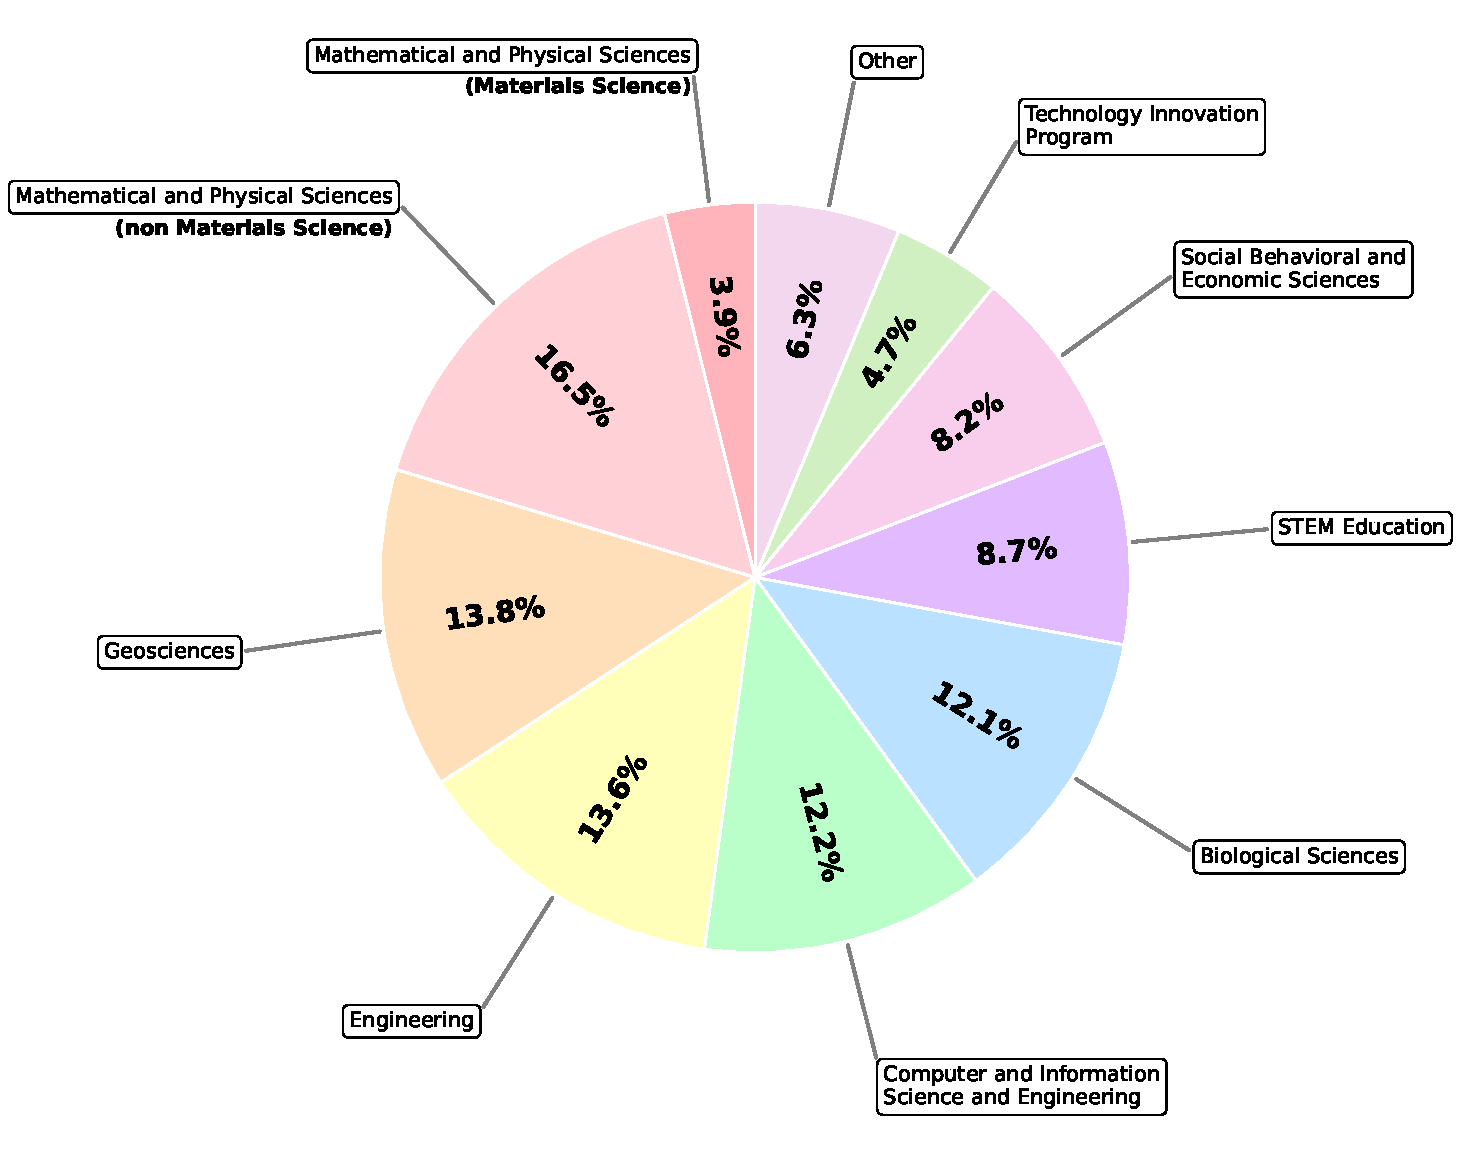
\includegraphics[width=1\linewidth]{images/directorate_distribution_with_materials.pdf}
    \caption{Distribution of awards areas as represented by the \NSF~directorates in \DatasetName, illustrating the breadth and comprehensiveness of scientific claims in our dataset. The \DatasetNameMatSci~subset spanning all of materials science awards represents 3.9\% of the entire dataset.}
    \label{fig:award-distribution}
\end{figure}
\begin{figure*}[h!]
    \centering
    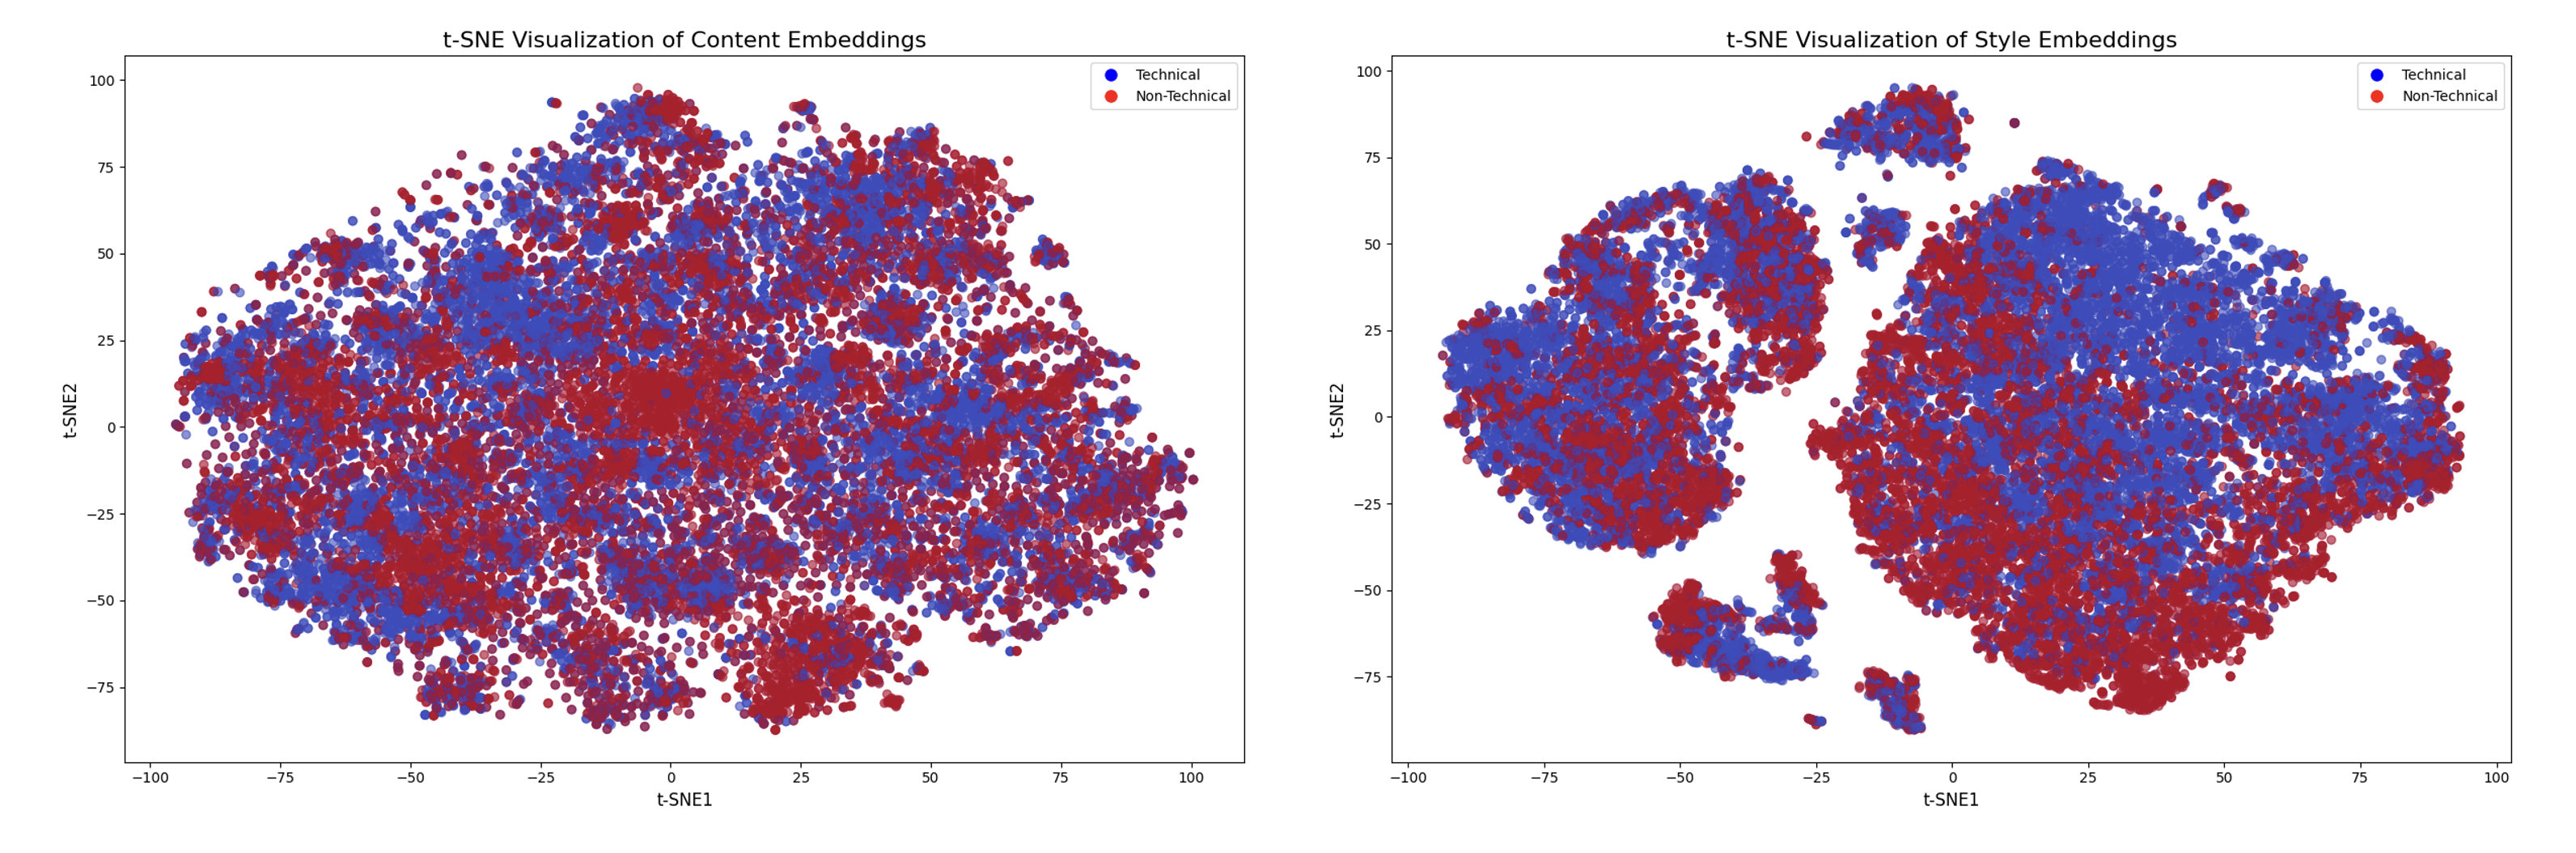
\includegraphics[width=1\linewidth]{images/tsne-specter-stel.png}
    \caption{The t-SNE plot of comparing content embeddings from SPECTER \cite{cohan-etal-2020-specter} and style embeddings from STEL \cite{patel2025} for technical and non-technical abstracts in \DatasetNameMatSci. The somewhat clear separation between technical and non-technical abstracts when using style embeddings indicate marked stylistic differences between the two kinds abstracts.}
    \label{fig:tsne-specter-stel}
\end{figure*}
\section{Building \DatasetName}

\subsection{Data Collection}
We downloaded the entire NSF Awards database\footnote{\url{https://www.nsf.gov/awardsearch/advancedSearch.jsp}} in XML format, containing more than 0.5 million awards from 1970 through September 2024. After parsing, we obtained 412,155 parseable awards, which we call \DatasetName. While we leave comprehensive processing of the full \DatasetName~dataset for future versions of this preprint, we make the parsed awards available for anyone immediately interested\footnote{Available at \url{https://huggingface.co/darpa-scify}}.

In this paper, we focus on all awards from the Division of Materials Research (DMR), which is responsible for most materials science awards at the NSF.  This subset, called \DatasetNameMatSci, contains 16,031 awards, representing approximately 3.2\% of the entire NSF awards database. We chose materials science as our initial focus due to its interdisciplinary nature and technological importance.

\subsection{Data Processing}

As Figure~\ref{fig:sample-record} illustrates, each record in  \DatasetNameMatSci~typically contains:
\begin{enumerate}[noitemsep,topsep=0pt]
\item Award ID, title, and year.
\item Directorate and division information
\item Technical abstract
\item Non-technical abstract (present in $\sim$81\% of awards)
\item Scientific claims made in the abstracts
\item Investigation proposals in the abstracts
\item Publications resulting from the grant (when available)
\end{enumerate}

The practice of updating awards with resulting publications is relatively recent, primarily occurring from 2014 onwards. For awards where publications are present, we extracted the DOIs and resolved them to obtain titles, abstracts, and publication URLs.

\subsection{Claim and Investigation Proposal Extraction}

To extract scientific claims and investigation proposals from the award abstracts, we developed a zero-shot prompting approach using Anthropic's Claude-3.5\footnote{\texttt{Claude-3.5-Sonnet-20240620} accessed between Sep-Oct. 2024, to be specific} model. Our prompt instructed the model to identify two types of statements:

\begin{enumerate}[noitemsep,topsep=0pt]
\item \textbf{Verifiable claims}: Statements that the abstract claims to be true or states as assumptions, either explicitly or implicitly.
\item \textbf{Investigation proposals}: Forward-looking statements that propose specific research activities as part of the award.
\end{enumerate}

We structured the prompt to return a JSON object containing the award ID, technical abstract, non-technical abstract, a list of verifiable claims, and a list of investigation proposals. To maintain consistency and quality, we set temperature to zero for all extractions. See Appendix~\ref{appendix:claude-claim-extraction} for the exact prompt and Appendix~\ref{appendix:claim-IP-examples} for sample claims and investigation proposals.

We performed qualitative experiments with several prompt variants and our analysis showed that jointly extracting claims and investigation proposals helped maintain the relevance of extracted claims. When claims were extracted without also extracting investigation proposals, the model often confused forward-looking statements about proposed investigations as factual claims.

\section{Dataset Analysis}
\paragraph{\DatasetName} The full dataset contains 412,155 award abstracts spanning from 1970 to 2024, with an estimated 2.8 million scientific claims and corresponding investigation proposals.

\paragraph{\DatasetNameMatSci} This materials science subset, which is the focus of this preprint, contains:
\begin{itemize}[noitemsep,topsep=0pt]
\item 16,042 awards with each with a technical and non-technical abstract
\item 114K extracted scientific claims (average of $7\pm2$ claims per abstract-pair)
\item 145K extracted investigation proposals (average of $9\pm3$ proposals per abstract-pair)
\item 2,953 awards with linked publications (18.4\% of the dataset). Such awards had anywhere between 1 -- 4 publications.
\end{itemize}

\subsection{Technical vs. Non-Technical Abstracts}
We investigated the differences between technical and non-technical abstracts in our dataset. Using a symmetric BLEU score to measure textual similarity between paired abstracts, we found that only 202 (1.5\%) out of 13,025 technical/non-technical abstract pairs had a similarity score greater than 0.6, suggesting that the non-technical abstracts are not simply copied from the technical abstracts.

Since grant abstracts are previously unexamined in literature, we further investigated the stylistic differences between technical and non-technical abstracts using pre-trained document embedding models. Figure~\ref{fig:tsne-specter-stel} compares content embeddings from SPECTER \cite{cohan-etal-2020-specter} and style embeddings from STEL \cite{patel2025}. Using these embeddings with a linear SVM classifier, we achieved F1 scores of 90.99 (SPECTER), 88.42 (STEL), and 89.99 (concatenated), demonstrating that the abstracts are distinguishable both in content and style.

\section{Tasks, Metrics, and Experiments}

We designed three NLP tasks to evaluate the utility of our dataset and establish baseline performance:

\begin{itemize}[noitemsep, wide, labelwidth=!, labelindent=0pt]
\item [\textbf{Task 1 -}] \textbf{Non-technical Abstract Generation:} Converting technical abstracts into non-technical language.
\item [\textbf{Task 2 -}]\textbf{Abstract to Scientific Claims:} Extracting scientific claims from abstracts.
\item [\textbf{Task 3 -}]\textbf{Abstract to Investigation Proposals:} Extracting investigation proposals from abstracts.
\end{itemize}

\subsection{Data Preparation}

Starting with 16,042 processed entries in \DatasetNameMatSci, we removed near-duplicates in technical and non-technical abstracts using trigram Jaccard similarity (threshold > 0.9), resulting in 11,569 data points. We further filtered cases where character-level 10-gram similarity between an entry's technical and non-technical abstracts exceeded 0.6, yielding 11,141 final data points. We split this dataset into train/validation/test sets with 8,641/500/2,000 examples, respectively.

\begin{table}[t]
\centering
\small
\begin{tabular}{lll}
\toprule
Metric & Mistral & Qwen\\
\midrule
BERTScore-P & 0.8563 \textcolor{darkgreen}{(+0.38\% $\uparrow$)} & 0.8459 \textcolor{darkgreen}{(+0.98\% $\uparrow$)} \\
BERTScore-R    & 0.8555 \textcolor{darkgreen}{(+0.30\% $\uparrow$)} & 0.8597 \textcolor{darkgreen}{(+1.61\% $\uparrow$)} \\
BERTScore-F1        & \textbf{0.8561} \textcolor{darkgreen}{(+0.36\% $\uparrow$)} & 0.8437 \textcolor{darkgreen}{(+0.75\% $\uparrow$)} \\
ROUGE1              & 0.2000 \textcolor{darkgreen}{(+2.58\% $\uparrow$)} & 0.1978 \textcolor{darkgreen}{(+1.98\% $\uparrow$)} \\
ROUGE2              & 0.0198 \textcolor{darkgreen}{(+4.76\% $\uparrow$)} & 0.0210 \textcolor{darkgreen}{(+3.89\% $\uparrow$)} \\
ROUGE-L             & 0.1273 \textcolor{darkgreen}{(+2.96\% $\uparrow$)} & 0.1466 \textcolor{darkgreen}{(+0.65\% $\uparrow$)} \\
ROUGE-L-sum         & 0.2166 \textcolor{darkgreen}{(+2.45\% $\uparrow$)} & 0.2078 \textcolor{darkgreen}{(+1.66\% $\uparrow$)} \\
\bottomrule
\end{tabular}
\caption{Finetuning performance for \texttt{Mistral-7B-instruct-v0.3}
 and \texttt{Qwen2.5-7B-Instruct}
 models for Technical abstract to Non-technical abstract translation (Task 1), with relative improvements over the corresponding unfinetuned model indicated in \textcolor{darkgreen}{green}. Error bars for all metrics at 95\% confidence intervals range between 0.0000--0.0025. Mistral model outperforms Qwen on almost all metrics for this task regardless of finetuning. We note that the percent changes, while statistically significant, are modest for this task indicating an excellent out-of-the-box performance that's challenging to improve upon.}
\label{tab:eval_tech2nontech}
\end{table}

\subsection{Models and Training}

To explore the four tasks, we finetuned two 7B parameter language models:
\begin{itemize}[noitemsep,topsep=0pt]
\item \texttt{Mistral-7B-instruct-v0.3}~\cite{jiang2023mistral7b}
\item \texttt{Qwen2.5-7B-Instruct}~\cite{qwen2}
\end{itemize}

For fine-tuning, we used LoRA~\cite{hu2021lora} with rank=128, lora\_alpha=64 and a learning rate of 1e-5 scheduled linearly. We updated the query, key, value, and output projection layers, as well as MLP gate, up, and down projections. We ran the finetuning on an A100 GPU for 3 epochs, 100 warmup steps, and a batch size of 2 with 4 accumulated steps. 

\subsection{Evaluation Metrics}

For Task 1 -- abstract generation -- we employed a comprehensive evaluation framework using both BERTScore~\cite{zhang2020bertscore} and ROUGE~\cite{lin-2004-rouge} metrics to assess the quality of generated non-technical abstracts. This combination enables us to capture both lexical overlap and structural similarity through the ROUGE variants, while BERTScore provides insights into semantic alignment between the generated texts and reference abstracts. Incorporating such multi-viewed metrics\footnote{For BERTScore we report precision, recall and F1, and for ROUGE we report ROUGE-1, ROUGE-2, ROUGE-L, and ROUGE-L-sum.} ensures that the evaluation reflects not only the presence of key words and phrases but also the underlying meaning and narrative coherence of the abstracts.

For Task 2 -- claim extraction -- we developed a novel evaluation approach using LLM-based comparisons. Previous methods for claim evaluations focused on comparing a single claim against a single document. See ~\citet{tang-etal-2024-minicheck}, for example. However, our setting required evaluating a set of extracted claims against a gold set of claims.
% \footnotetext[3]{We determine repeats and near-repeats in the generation by thresholding cosine similarity calculated over a TF-IDF representation of the generated claims.}


Towards that end, we defined a boolean function $\mathbf{\Phi}_{\textrm{claim}}$ using \texttt{GPT-4o-mini} with zero-shot prompting to determine whether a generated claim is supported by a gold standard claim. See Appendix~\ref{appendix:phi_claim} for prompt details. Using this function, we calculated precision and recall as follows:
\begin{equation*}
\left.\begin{aligned}
\text{Precision}&=&\frac{1}{|S|} \sum_{c \in S} \max_{g \in G} \mathbf{\Phi}_{\textrm{claim}}(c, g)\\
\text{Recall}&=&\frac{1}{|G|} \sum_{g \in G} \max_{c \in S} \mathbf{\Phi}_{\textrm{claim}}(g, c)
\end{aligned}\right.
\end{equation*}
\noindent where $S$ is the set of claims generated from the finetuned model, after removal of any repeats/near-repeats
% \footnotemark[3],
\footnote{We determine repeats and near-repeats in the generation by thresholding cosine similarity calculated over a TF-IDF representation of the generated claims.},
 and $G$ is the gold standard set. We note that this is a variant of precision/recall metrics defined for image captioning in~\cite{deitke2024molmo}, however unlike ~\citeauthor{deitke2024molmo}, we explicitly use $\mathbf{\Phi}_{\textrm{claim}}$ in computing both precision and recall. This is necessary as we need to accurately penalize any spurious claims generated by the finetuned model.

Analogously, for Task 3 -- extraction of investigation proposals -- we define precision and recall similarly but use a different pairwise boolean judge function $\mathbf{\Phi}_{\textrm{IP}}$ \textit{mutatis mutandis}. See Appendix~\ref{appendix:phi_IP} for prompt details.


\section{Results}

\subsection{Non-technical Abstract Generation}
Table \ref{tab:eval_tech2nontech} shows the results for Task 1. Both Mistral and Qwen models demonstrated strong performance, with fine-tuning providing modest improvements. The Mistral model outperformed Qwen on almost all metrics, achieving a BERTScore-F1 of 0.8561 after fine-tuning (+0.36\% relative improvement). ROUGE scores were generally low (0.01-0.22), reflecting the stylistic differences between technical and non-technical abstracts.


\subsection{Scientific Claim Extraction}

\begin{table}[h]
\centering
\small
\begin{tabular}{lll}
\toprule
Metric & Mistral & Qwen \\
\midrule
Precision
 & 0.7450 \textcolor{darkgreen}{\,(+116.7\% $\uparrow$)} 
 & 0.6839 \textcolor{darkgreen}{\,(+107.1\% $\uparrow$)} \\
Recall 
 & 0.7098 \textcolor{darkgreen}{\,(+59.5\% $\uparrow$)} 
 & 0.6611 \textcolor{darkgreen}{\,(+7.8\% $\uparrow$)} \\
F1 
 & 0.7097 \textcolor{darkgreen}{\,(+101.8\% $\uparrow$)} 
 & 0.6541 \textcolor{darkgreen}{\,(+63.3\% $\uparrow$)} \\
%\textbf{Precision} & 0.3438 $\pm$ 0.0053 & \textbf{0.7450 $\pm$ 0.0042} & 0.3302 $\pm$ 0.0044 & 0.6839 $\pm$ 0.0048 \\
%\textbf{Recall} & 0.4451 $\pm$ 0.0055 & \textbf{0.7098 $\pm$ 0.0044} & 0.6131 $\pm$ 0.0055 & 0.6611 $\pm$ 0.0045 \\
%\textbf{F1} & 0.3516 $\pm$ 0.0050 & \textbf{0.7097 $\pm$ 0.0038} & 0.4005 $\pm$ 0.0047 & 0.6541 $\pm$ 0.0043 \\
\bottomrule
\end{tabular}
\caption{Finetuning performance for \texttt{Mistral-7B-instruct-v0.3}
 and \texttt{Qwen2.5-7B-Instruct}
 models for Claim Extraction from abstracts (Task 2), with relative improvements over the corresponding unfinetuned model indicated in \textcolor{darkgreen}{green}. Error bars for all metrics at 95\% confidence intervals range between 0.0038--0.0055. Mistral model outperforms Qwen on almost all metrics for this task regardless of finetuning. We note the large positive percent changes, sometimes improvements as large as 2x, indicate finetuning is indispensable for claim extraction. Mistral model outperforms Qwen on almost all metrics for this task.}
\label{tab:eval_technontech2claims}
\end{table}

For Task 2 (claim extraction), fine-tuning yielded substantial improvements. As shown in Table \ref{tab:eval_technontech2claims}, the fine-tuned Mistral model achieved a precision of 0.7450 (+116.7\% relative improvement), recall of 0.7098 (+59.5\%), and F1 of 0.7097 (+101.8\%). The Mistral model consistently outperformed Qwen, though both showed significant benefits from fine-tuning.

\subsection{Investigation Proposal Extraction}
Similarly, Task 3 (proposal extraction) showed dramatic improvements with fine-tuning. As shown in Table \ref{tab:eval_technontech2ip}, the Mistral model achieved a precision of 0.7351 (+18.24\%), recall of 0.7539 (+127.24\%), and F1 of 0.7261 (+90.97\%) after fine-tuning. The relative improvements were even larger for the Qwen model, though Mistral still performed better overall.
\begin{table}[h!]
\centering
{\small
\begin{tabular}{lll}
\toprule
Metric & Mistral & Qwen\\
\midrule
Precision
 & 0.7351 \textcolor{darkgreen}{(+18.24\% $\uparrow$)} 
 & 0.7245 \textcolor{darkgreen}{(+70.07\% $\uparrow$)} \\
Recall 
 & 0.7539 \textcolor{darkgreen}{(+127.24\% $\uparrow$)} 
 & 0.6865 \textcolor{darkgreen}{(+81.57\% $\uparrow$)} \\
F1
 & 0.7261 \textcolor{darkgreen}{(+90.97\% $\uparrow$)} 
 & 0.6827 \textcolor{darkgreen}{(+112.60\% $\uparrow$)} \\
%\textbf{Precision} & 0.6217 $\pm$ 0.0070 & \textbf{0.7351 $\pm$ 0.0041} & 0.4426 $\pm$ 0.0073 & 0.7245 $\pm$ 0.0045 \\
%\textbf{Recall} & 0.3317 $\pm$ 0.0047 & \textbf{0.7539 $\pm$ 0.0040} & 0.3781 $\pm$ 0.0051 & 0.6865 $\pm$ 0.0046 \\
%\textbf{F1} & 0.3802 $\pm$ 0.0053 & \textbf{0.7261 $\pm$ 0.0036} & 0.3211 $\pm$ 0.0054 & 0.6827 $\pm$ 0.0041 \\
\bottomrule
\end{tabular}
\caption{Finetuning performance for \texttt{Mistral-7B-instruct-v0.3}
 and \texttt{Qwen2.5-7B-Instruct}
 models for extraction of Investigation Proposals from award abstracts (Task 3), with relative improvements over the corresponding unfinetuned model indicated in \textcolor{darkgreen}{green}. Error bars for all metrics at 95\% confidence intervals range between 0.0036--0.0073. Mistral model outperforms Qwen on almost all metrics for this task regardless of finetuning. We note the large positive percent changes, sometimes improvements as large as 2x, indicate finetuning is indispensable for this task. Mistral model outperforms Qwen on almost all metrics for this task.}
\label{tab:eval_technontech2ip}
}
\end{table}

\section{Discussion and Conclusion}

In this paper, we introduced \DatasetName, a large-scale dataset of scientific claims and investigation proposals extracted from NSF grant abstracts. Our dataset is significantly larger than previous scientific claim datasets, with an estimated 2.8 million claims across all NSF fields and 114,000 claims in materials science alone.

Our experiments demonstrated that fine-tuning language models on this dataset substantially improves their ability to extract both scientific claims and investigation proposals. The strong performance gains (often exceeding 100\% relative improvement) suggest that grant abstracts contain structured information, particularly claims and investigation proposals, that models can learn to extract systematically.

The analysis of technical versus non-technical abstracts revealed interesting stylistic differences, suggesting potential applications in science communication, HCI, and accessibility. The presence of both claims and investigation proposals in the same documents provides a unique opportunity for future work to study the relationship between what scientists claim to know and what they propose to discover.

\DatasetName~offers several advantages for scientific claim verification research:
\begin{enumerate}[noitemsep,topsep=0pt]
\item \textbf{Scale}: It contains orders of magnitude more claims than previous datasets.
\item \textbf{Quality}: Award grants that pass through the \NSF's high-quality expert review process provides a filter for claim quality.
\item \textbf{Longitudinal coverage}: The dataset spans from 1970 to 2024, enabling temporal analyses.
\item \textbf{Cross-disciplinary scope}: It covers all scientific domains funded by NSF.
\item \textbf{Linked outcomes}: For recent grants, the associated publications allow tracking from proposal to result.
\end{enumerate}

To foster research on large-scale claim extraction, we are releasing our datasets and trained models:
\begin{itemize}[noitemsep,topsep=0pt]
\item \DatasetNameMatSci: Materials Science subset with extracted claims, investigation proposals, and resolved publication information.
\item \DatasetName: Similar in content to~\DatasetNameMatSci, but a larger superset spanning all of NSF awards database. The key difference is the claims and investigation proposals are extracted from our finetuned models instead of frontier LLMs.
\item Our best finetuned model checkpoints for extraction of claims and investigation proposals on HuggingFace\footnote{at \url{https://huggingface.co/darpa-scify}}.
\end{itemize}

Future work could expand to other funding agencies, develop specialized claim verification systems for grant proposals, and explore the relationship between proposed investigations and eventual research outcomes.

\section*{Acknowledgments}
The authors would like to acknowledge the Defense Advanced Research Projects Agency (DARPA) SciFy program (Agreement No. \texttt{HR00112520300}) for funding this research. We also thank the National Science Foundation (NSF) for making award data publicly available, enabling this research. Any opinions, findings and conclusions or recommendations expressed in this material are those of the author(s) and do not necessarily reflect the official policy, position, or views of the National Science Foundation, DARPA, the Department of Defense, or the U.S. Government.

% Bibliography entries for the entire Anthology, followed by custom entries
%\bibliography{anthology,custom}
% Custom bibliography entries only
\bibliography{main}

\clearpage

\section*{Appendix}

\appendix

\section{Complete Prompt for Extracting Claims and Investigation Proposals}
\label{appendix:claude-claim-extraction}
\begin{mdframed}[backgroundcolor=blue!20]
\noindent You are an expert materials science researcher. Given an input JSON description of an NSF material science award abstract, parse out the technical and nontechnical abstracts, and identify the verifiable claims and research/investigation proposals the abstract makes. Be thorough. Answer in the following JSON format:
\begin{lstlisting}
{
  "award_id": "", // copied from input
  "technical_abstract": ""  // technical abstract if present, otherwise contents of the abstract field in the input
  "non_technical_abstract": /non-technical abstract if present, otherwise empty
  "verifiable_claims": [ // list of strings
  ],
  "investigation_proposals":  [ // list of strings
  ],
}    
\end{lstlisting}

\noindent verifiable\_claims are statements that the abstract claims to be true or states as an assumption explicitly or implicitly. \\
\noindent investigation\_proposals are forward-looking statements that the abstract proposals to investigate as a part of this award. \\
\noindent Ensure that the output is in JSON format and that the JSON is valid.
\end{mdframed}
We manually tested the prompt with a few award abstracts to make sure it was optimal for this task.

\section{Prompt for Task 2 evaluation function $\mathbf{\Phi}_{\textrm{claim}}$}
\label{appendix:phi_claim}
\begin{mdframed}[backgroundcolor=blue!20]
\noindent Check two scientific claims c1 and c2, if c1 is supported by c2. If c2 includes all the evidences for c1, but also includes additional content, then it should still be supported (YES). If not all information of c1 is included in c2, or if c2 contains information that conflicts with information in c1, then it should be unsupported (NO). Answer only as a YES or NO.\\
\noindent c1: \{c1\}\\
\noindent c2: \{c2\}
\end{mdframed}

\section{Prompt for Task 3 evaluation function $\mathbf{\Phi}_{\textrm{IP}}$}
\label{appendix:phi_IP}
\begin{mdframed}[backgroundcolor=blue!20]
\noindent Check two investigation proposals c1 and c2, if c1 is supported by c2. If c2 includes all the investigations proposed by c1, but also includes additional proposals, then it should still be supported (YES). If not all proposed investigations by c1 is included in c2, or if c2 contains investigation actions that conflict with investigation actions in c1, then it should be unsupported (NO). Answer only as a YES or NO.\\
\noindent c1: \{c1\}\\
\noindent c2: \{c2\}
\end{mdframed}

\section{Examples of Extracted Claims and Investigation Proposals}
\label{appendix:claim-IP-examples}
Tables~\ref{tab:claim-examples} and~\ref{tab:ip-examples} provide a sampling of the extracted claims and investigation proposals. 

\rowcolors{2}{gray!10}{white}
\begin{table*}[h]
\centering
    \begin{tabular}{lp{5cm}p{8cm}}
    \toprule
    \rowcolor{white} 
         \textbf{Award ID} & \textbf{Title} & \textbf{Extracted Claims}\\
         \midrule
         \href{https://www.nsf.gov/awardsearch/showAward?AWD_ID=2324035&HistoricalAwards=false}{2324035} & DMREF: Developing and Harnessing the Platform of Quasi-One-Dimensional Topological Materials for Novel Functionalities and Devices & \begin{minipage}{\linewidth}
\begin{lstlisting}
[
    "Topological insulators are electrically insulating in the bulk but host conductive surface states that are immune to impurities.",
    "Current TI materials face critical challenges that limit their potential.",
    "Quasi-1D structures promise to overcome challenges faced by current TI materials.",
    "Most identified topological insulators are either strongly bonded bulk materials or layered van der Waals materials.",
    ...
]
\end{lstlisting}
\end{minipage} \\
         \href{https://www.nsf.gov/awardsearch/showAward?AWD_ID=9814055&HistoricalAwards=false}{9814055} & Kinks and Surface Potentials & \begin{minipage}{\linewidth}
\begin{lstlisting}
[
    "Atomically flat terraced surfaces for thin TEM samples can be prepared under moderate (10-7 Torr) vacuum conditions by annealing in oxygen or vacuum for materials such as sapphire, SiC and MgO.",
    "\"Forbidden\" Bragg reflections arise from the stacking fault between partial dislocations.",
    "The surface potential is critical for chemical reactions at surfaces, adsorption, catalysis, epitaxy, diffusion bonding process, oxidation, and semiconductor crystal growth.",
    ...
]
\end{lstlisting}
\end{minipage} \\
         \href{https://www.nsf.gov/awardsearch/showAward?AWD_ID=0821136&HistoricalAwards=false}{0821136} & MRI: Acquisition of an Imaging Spherical Aberration Corrector and a Lorentz Lens for Magnetic Materials Characterization & \begin{minipage}{\linewidth}
\begin{lstlisting}
[
    "The attainable spatial resolution of uncorrected Lorentz instruments is in the range 10-15 nm.",
    "Delocalization effects cause significant image blurring in uncorrected Lorentz microscopes.",
    "Recent developments in aberration correction make it possible to correct the spherical aberration of a Lorentz lens.",
    "The size of written bits in state-of-the-art magnetic recording media is comparable to the magnetic resolution of uncorrected Lorentz microscopes.",
    "Transmission electron microscopes have suffered from lens aberration since their invention in the 1930s.",
    "The Hubble space telescope suffered from a similar aberration when first launched.",
    ...
]
\end{lstlisting}
\end{minipage} \\
    \bottomrule
    \end{tabular}
    \caption{A sample of extracted claims from the \DatasetNameMatSci~dataset. Award IDs are hyperlinked to the NSF's Award database.}
    \label{tab:claim-examples}
\end{table*}


\rowcolors{2}{gray!10}{white}
\begin{table*}[h]
\centering
    \begin{tabular}{lp{5cm}p{8cm}}
    \toprule
    \rowcolor{white} 
         \textbf{Award ID} & \textbf{Title} & \textbf{Extracted Investigation Proposals}\\
         \midrule
         \href{https://www.nsf.gov/awardsearch/showAward?AWD_ID=2324035&HistoricalAwards=false}{2324035} & DMREF: Developing and Harnessing the Platform of Quasi-One-Dimensional Topological Materials for Novel Functionalities and Devices & \begin{minipage}{\linewidth}
\begin{lstlisting}
[
    "Predict, design, synthesize, and control topological phases in quasi-1D topological materials.",
    "Design and demonstrate emergent materials, functionalities, and devices, including moir\'e quasi-1D TIs, stable and high temperature quantum spin Hall (QSH) insulators, and quantum intelligent sensors.",
    "Expand research to include other selected quasi-1D materials families through collaborations.",
    "Discover or realize novel topological materials and phases.",
    "Study topological phase transitions and control.",
    "Investigate room-temperature QSH effect.",
    ...
]
\end{lstlisting}
\end{minipage} \\
         \href{https://www.nsf.gov/awardsearch/showAward?AWD_ID=9814055&HistoricalAwards=false}{9814055} & Kinks and Surface Potentials & \begin{minipage}{\linewidth}
\begin{lstlisting}
[
    "Observe dislocation kinks by atomic resolution TEM in materials such as sapphire, SiC and MgO.",
    "Use \"forbidden\" Bragg reflections to form lattice images without surface noise.",
    "Determine which process (kink formation, kink migration or obstacles along the dislocation line) limits kink (and hence dislocation) velocity, for given conditions of temperature and stress.",
    "Extend quantitative convergent-beam TEM measurements of bonding in crystals to the RHEED geometry to refine the electrostatic potential extending into the vacuum from ceramic surfaces.",
    "Measure modifications to the surface potential resulting from the deposition of a monolayer or more of atoms.",
    ...
]
\end{lstlisting}
\end{minipage} \\
         \href{https://www.nsf.gov/awardsearch/showAward?AWD_ID=0821136&HistoricalAwards=false}{0821136} & MRI: Acquisition of an Imaging Spherical Aberration Corrector and a Lorentz Lens for Magnetic Materials Characterization & \begin{minipage}{\linewidth}
\begin{lstlisting}
[
    "Acquire an imaging spherical aberration corrector and a Lorentz lens for magnetic materials characterization.",
    "Add these components to an existing FEI Titan 80-300 TEM.",
    "Bring the spatial resolution in Lorentz mode down to less than 1 nm, with negligible delocalization effects.",
    "Enable direct quantitative study of magnetic features at a length scale of around 1 nm.",
    "Obtain new scientific results on material systems for which these observations were previously impossible.",
    "Impact a large number of research groups within CMU, as well as collaborations with local industry and several national laboratories.",
    ...
]
\end{lstlisting}
\end{minipage} \\
    \bottomrule
    \end{tabular}
    \caption{A sample of extracted investigation proposals from the \DatasetNameMatSci~dataset. Award IDs are hyperlinked to the NSF's Award database.}
    \label{tab:ip-examples}
\end{table*}

\end{document}

